% Editable source for the spatial partition in kdt.md.
% From this directory, regenerate with:
% latex -interaction=nonstopmode -halt-on-error kdt-1.tex
% dvisvgm --no-fonts --exact --bbox=papersize --output=kdt-1.svg kdt-1.dvi
\documentclass[tikz,border=5pt]{standalone}
\usepackage{lmodern}
\definecolor{xsplit}{HTML}{D94B4B}
\definecolor{ysplit}{HTML}{494AC7}
\begin{document}
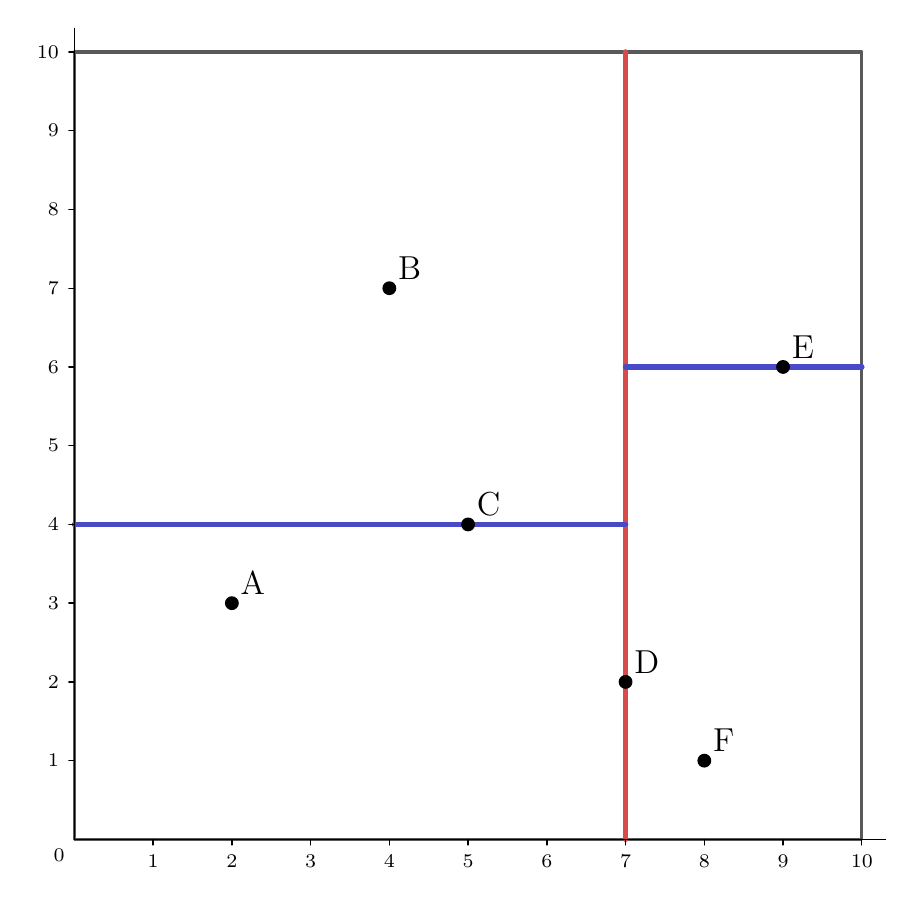
\begin{tikzpicture}[x=1cm,y=1cm,font=\large,line cap=round,line join=round]
  % The root D splits at x=7. Its children C and E split at y=4
  % and y=6 within their respective regions. Leaves do not split further.
  \draw[black!65,line width=1.2pt] (0,0) rectangle (10,10);
  \draw[xsplit,line width=2pt] (7,0) -- (7,10);
  \draw[ysplit,line width=2pt] (0,4) -- (7,4);
  \draw[ysplit,line width=2pt] (7,6) -- (10,6);

  \draw[line width=0.5pt] (0,0) -- (10.3,0);
  \draw[line width=0.5pt] (0,0) -- (0,10.3);
  \node[below left,font=\scriptsize] at (0,0) {0};
  \foreach \tick in {1,...,10} {
    \draw[line width=0.5pt] (\tick,0) -- (\tick,-0.07)
      node[below,font=\scriptsize] {\tick};
    \draw[line width=0.5pt] (0,\tick) -- (-0.07,\tick)
      node[left,font=\scriptsize] {\tick};
  }

  % These six coordinates also label the nodes in kdt-2.tex.
  \foreach \name/\px/\py in {A/2/3,B/4/7,C/5/4,D/7/2,E/9/6,F/8/1} {
    \fill (\px,\py) circle[radius=2.5pt];
    \node[above right=3pt,inner sep=0pt] at (\px,\py) {\name};
  }
\end{tikzpicture}
\end{document}
